

\section{System Architecture}

\begin{figure}[ht!]
\centering
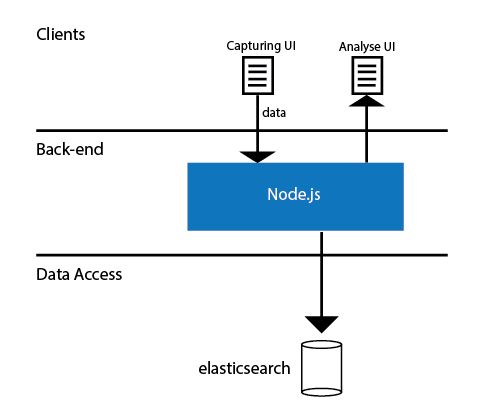
\includegraphics[width=100mm]{images/general/arhitecture.png}
\caption{Overall architecture of the system }
\label{overflow}
\end{figure}

The system architecture can be layered in to three layers; client, back-end, database. The control flow flows from the clients requesting something or inserting data, to the back-end and to the third layer, the database, and back up again in reverse order. 

\subsubsection{Interface}

The Soccer Analytic tool has one user interface - the web browser interface. Both the input and the analytic interface can be reached from this single web browser interface.

\subsubsection{Back-end}

The back-end is the middle layer between the client and the storage. Its main task is to serve static files to the clients, handle data insertions or handling web request by mapping them to database operations. New data insertions will possible be inserted into several database indexes. The back-end will then ensure that all indexes are updated before returning success to the client.

\subsubsection{Storage}

The storage layers task is to persist data and handle search queries on the data. It consist of several indexes that each store a part of domain the model. 

\subsection{Domain model}

The domain model is based around matches. All attacks is wrapped into a match root. Attacks can be seen as subdocuments of the match document. Inside the attacks all passes lies with other information. This gives a easy way of understanding how all the data is related together. Below is a complete example of how it all is structured. The number of attacks and passes is stripped down to one in the example.

\lstinputlisting{domainmodel.js}

\section{Implementation details}

\begin{figure}[ht!]
\centering
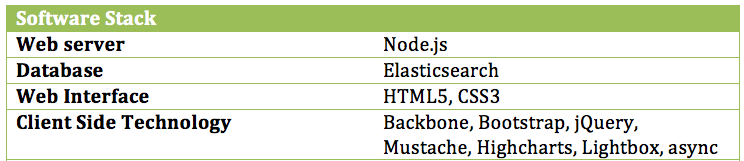
\includegraphics[width=100mm]{images/implementation/software_stack.png}
\caption{Software stack}
\label{overflow}
\end{figure}

\subsection{Storage}

The data storage is an elasticsearch database\footnote{http://www.elasticsearch.org/}. Elasticsearch is document oriented, schema less and works well with JSON\footnotemark. As our server is built on JavaScript working with JSON is easy. JSON-objects can be inserted right into the storage and elasticsearch will map fields and value accordingly, and make it available for search.
Elasticsearch takes advantages of embedded documents meaning we can store related data together. An attack is usually made up of several passes these can be stored as an embedded document in the attack document. Then all pases can be retrieved in one query when fetching an attack.

The main reason for using Elasticsearch is its search capability. In the starting phase of the project MongoDB \footnotemark was the storage engine. However as some aggregation queries was hard to figure out how to do a change to elasticsearch was made. It should be noted that MongoDB supports map reduce operations. With some extra work the queries causing problems could possible have been done with MongoDB. However, with elasticsearch you can in a single, simple to write query get counted how many passes all players for a team has played and received, the number of times all players has been the breakthrough-player in an attack, count type of attacks, count the most used zones for passing and finishing and so on. This makes it very easy and efficient to do queries for analyses on teams and players.

\footnotetext{http://www.json.org/}
\footnotetext{http://www.mongodb.org/}

\subsubsection{Indexes}

Indexes in much like tables in a relational database in the way that they is a container for data. An index stores documents which is a bunch of key/value pairs like JSON. You can let elasticsearch automatic analyze the field data or you can use mappings. For supporting querying on players and other fields where the value is more than one word, you have to tell elasticsearch that it is a multi field. For example searching for player name ''Stefan Johansen'' when the field is not set as multi field will give you two results and not one as you would expect.

In our project we have 5 different indexes. Team index which stores all the teams. Player index which stores all the players. Match index stores all data from a match including all attacks. Attack index stores information about attacks and last the pass index which stores passes. As may be noted there is data redundancy. You can argue that storage has become so cheap and if you can use a little bit extra space to gain performance you would do it. In this case it was done to be able to fully support aggregation functions on subdocuments.

\subsection{Back-end}

The back end is the middle-ware between the clients and the data layer. It exposes a RESTful\footnote{http://www.ibm.com/developerworks/webservices/library/ws-restful/} interface over HTTP for the client to communicate. A request coming in is transformed to a database query based on the resource it tries to access. On answer from the database the result is transformed before returning it to the client. 

Similar if the client sends new data for a match the middle-ware inserts the data into the appropriate indexes. The server will respond will HTTP status code 201 if all goes well or 400 on an error. The server uses HTTP code actively to tell the client the result of requests.

In principal, since the data input is generated in the web browser (with JavaScript), it could have been inserted right away into the database without going through an extra middleware. However, this limits us as we cant combine multiple queries by going through the back-end. Cleaning of data before serving to the client would neither be possible. Normally you also do validation of the data at the back-end before inserting into your database.

\subsubsection{API}

The API of the web server is listed in figure \ref{fig:api}.
\begin{figure}[ht!]
\centering
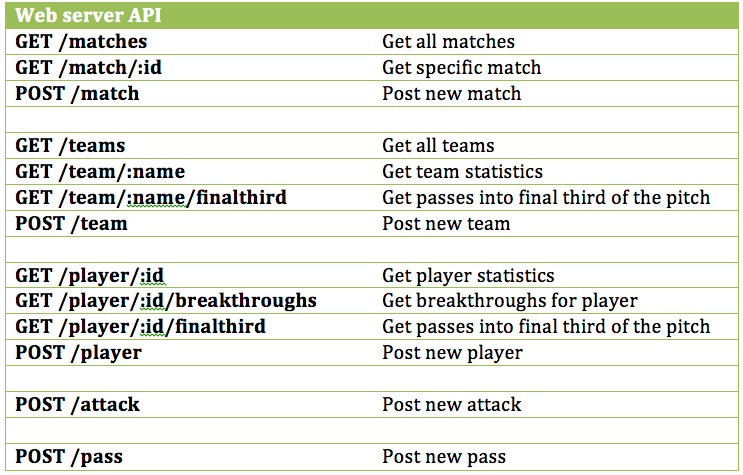
\includegraphics[width=100mm]{images/implementation/API.png}
\caption{Overview of the web servers API}
\label{fig:api}
\end{figure}

\subsection{Front-end}

Front end is consist of a single page JavaScript application using Backbone.js \footnotemark as under-supporting framework. Backbone uses a MVC model to structure the code. With Backbone your views will update automatic when data changes. In the following sections the architecture of the client and how different concepts is used will be described. 

\footnotetext{http://backbonejs.org/}

\begin{figure}[ht!]
\centering
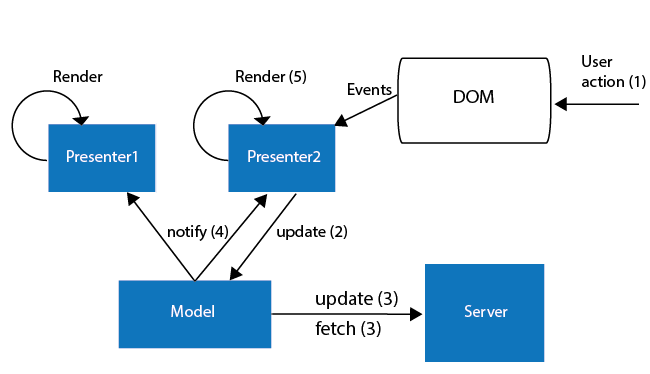
\includegraphics[width=150mm]{images/architecture/backbone_architecture.png}
\caption{Architecture of the client side}
\label{overflow}
\end{figure}

\subsubsection{Models}

Data is represented as models in backbone. The model has mainly two responsibilities. First is whenever a update on a models data occurs the model notifies the views that has subscribed for update events for that particular model. The second is that models is responsible for AJAX communication  with the back-end. An example is when a user registrates a new attack for a match. He fills out a form and press submit. Then a new Attack Model is created. Calling save on the instance of the model will send an AJAX post request to the server with the models data in the HTTP body.

Similar to a Attack Model we have Player Model that handles everything around players. When you click yourself into a players profile the model will fetch statistics from the back-end, notify the view that the data is ready, and the view will be rendered.

There is also a Match Model (fetching and registrating matches), Team Model (viewing statistics), and a Pass Model (saving passes). They work it the same way as the models described above.


\subsubsection{Views}

For a analytic toolkit to be useful a good UI is critical. Here several helper library is used to present the data. Highcharts.js\footnotemark  is a JavaScript library for illustrating graphs. A query on team generates a lot of statistics and rather than listing them up they are presented using charts. This also gives us the advantage of displaying several numbers for each player and plot it in the same graph. In figure \ref{fig:chart} the number of times a player has been involved in all attacks, number of passes into the final third of the pitch and the number of times a player has been the breakthrough-player is shown.

\footnotetext{http://www.highcharts.com/}

\begin{figure}[ht!]
\centering
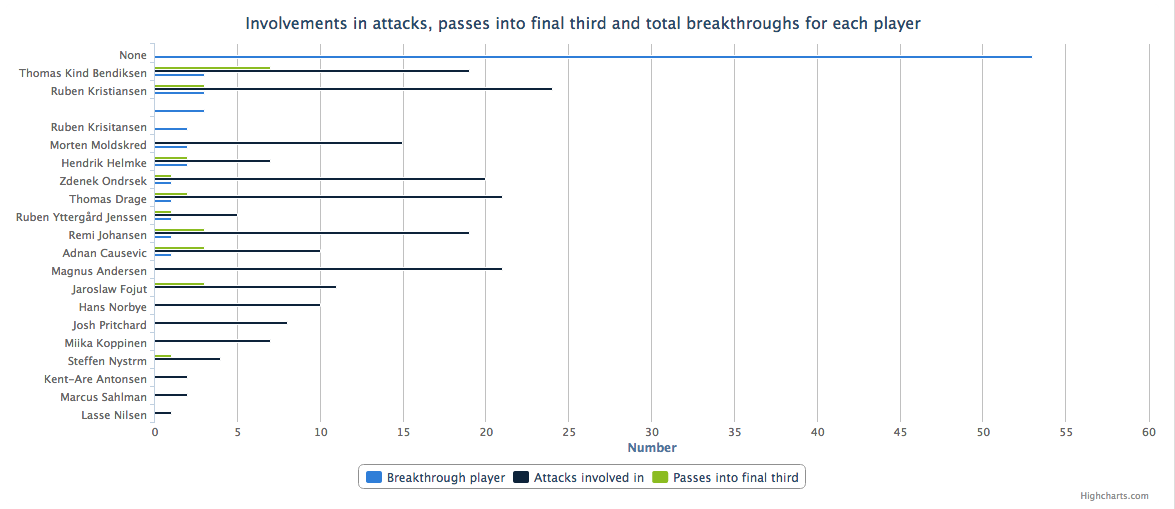
\includegraphics[width=100mm]{images/general/chart_passes.png}
\caption{Shows how the passing statistic is illustrated on the client by using Highcharts.js}
\label{fig:chart}
\end{figure}

Positional data is created using the a new feature of HTML5, canvas element. It lets you draw graphics on the fly in the web page. In this system it is used to create a element that symbols the different zones in our domain model. In the Team Model you have all zones with a number that symbols shots taken from that zone. This is then plotted into the respective zones.

\begin{figure}[ht!]
\centering
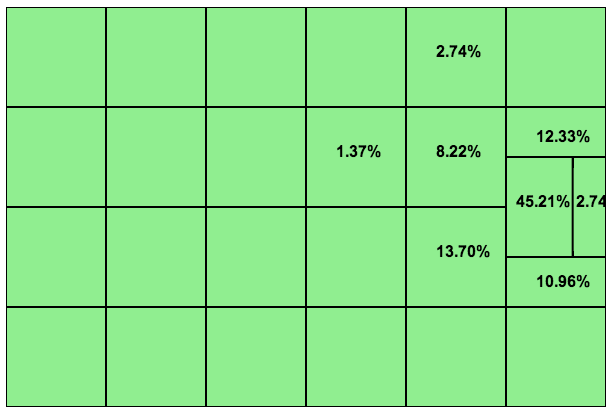
\includegraphics[width=85mm]{images/general/finishing_zones.png}
\caption{Illustrations of which zones the team has finished off their attacks from, with percent (team: Tromsø IL)}
\label{overflow}
\end{figure}

Backbone comes with a library Underscore.js\footnotemark that makes creating HTML pages with dynamic content easily. When you are rendering new content on the site you can insert data retried from a model dynamically into the HTML. In the example below the input is a an array of objects where each element in the array contains a key value pair 'name' : value. The html output of this will be a list of names.

\lstinputlisting{underscore_example.html}

\footnotetext{http://underscorejs.org/}

\subsubsection{Router}

A component not mentioned before that lies on the client is the router. The router is the glue that binds all the other moduels together. It handles the navigation between pages in the application. When users navigate on the page by clicking on links or buttons in a traditonal web page the back-end serves a new html page. In this page this click event is handled by a router module. The router model examins the URL request and routes the request to the mapped up view. The view is then responsible for calling fetch functions on the model and render the HTML.

ADD A SECOND ILLUSTRATION ADDNING THE ROUTER.

\subsection{Getting players and teams into the database}

Getting squads in a useful format like XML or JSON was harder than expected. On the norwegian football alliance's website you could download the squads for the current season only in PDF. Current squads is fetched from altomfotball.no, a website by the norwegian TV channel TV2. This is own python script meant to run only once to set up the database. For each team the script basically reads the HTML document with all players listed, parse out players name, and sends in to the web server.

MORE ON DEVELOPMENT PROCESS? How zone map changed etc. A change from Mongodb to elasticsearch


\subsection{Security}
Secturity is not taken into concern. This means anyone getting into the page can post new match data and add attacks. This could have been fixed by requiring a login before getting access to the site. 

